% Part: sets-functions-relations
% Chapter: infinite
% Section: hilberts-hotel
%
\documentclass[../../../include/open-logic-section]{subfiles}

\begin{document}

\olfileid{sfr}{infinite}{hilbert}
\olsection{હિલ્બર્ટની હોટેલ}

પ્રાકૃતિક સંખ્યાઓનો ગણ સ્પષ્ટપણે અનંત છે. તેથી, જો આપણે પ્રાકૃતિક
સંખ્યાઓને \emph{પહેલેથી જ માની લેવા} ન માગતા હોઈએ, તો આપણું પહેલું
પગલું પ્રાકૃતિક સંખ્યાઓનો પોતાનો ઉલ્લેખ કર્યા વિના અનંત ગણનું લક્ષણ
આપવાનું હોવું જોઈએ. ૧૯૨૪ના એક વ્યાખ્યાનમાં હિલ્બર્ટે રજૂ કરેલો આ એક
સુંદર અભિગમ છે. તેઓ આપણને કલ્પના કરવાનું કહે છે:
\begin{quote}
[\ldots] સાન્ત સંખ્યામાં ઓરડાઓ ધરાવતી એક હોટેલ. આ બધા ઓરડાઓમાં
બરાબર એક-એક મહેમાન રહેતો હોવો જોઈએ. હવે મહેમાનો કોઈક રીતે પોતાના
ઓરડા બદલે, [પણ] દરેક ઓરડામાં હજી વધુમાં વધુ એક જ વ્યક્તિ રહે એ રીતે,
તો એકેય ઓરડો ખાલી નહીં થાય અને હોટેલમાલિક આ રીતે નવા આવેલા મહેમાન
માટે નવી જગ્યા ઊભી કરી શકશે નહીં [\ldots
\textparagraph \ldots]

હવે આપણે ઠરાવીએ કે હોટેલમાં $1$, $2$, $3$, $4$, $5$, \dots એ રીતે
ક્રમાંકિત અનંત ઓરડાઓ હોય અને દરેકમાં બરાબર એક મહેમાન રહેતો હોય. નવો
મહેમાન આવે કે તરત માલિકે જૂના દરેક મહેમાનને તેના હાલના ક્રમાંક કરતાં
એક વધુ ક્રમાંકવાળા ઓરડામાં ખસેડવાનો જ રહે છે; ત્યારે નવા આવેલા મહેમાન
માટે ઓરડો~$1$ ખાલી થઈ જશે.
	\begin{center}
		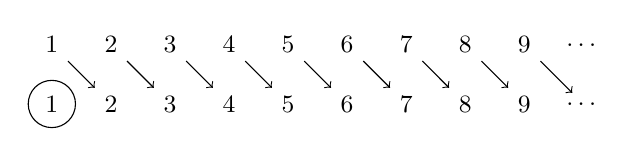
\begin{tikzpicture}[scale = .75]
		\foreach \x in {1, 2, 3, 4, 5, 6, 7, 8, 9}
		{
			\node (\x a) at (\x, 1) {\small{\x}};
			\node (\x b) at (\x, 2) {\small{\x}};
		}
		\node (dotsa) at (10, 1) {\small{\ldots}};
		\node (dotsb) at (10, 2) {\small{\ldots}};
		\draw[->] (1b)--(2a);
		\draw[->] (2b)--(3a);
		\draw[->] (3b)--(4a);
		\draw[->] (4b)--(5a);
		\draw[->] (5b)--(6a);
		\draw[->] (6b)--(7a);
		\draw[->] (7b)--(8a);
		\draw[->] (8b)--(9a);
		\draw[->] (9b)--(dotsa);
		\draw (1,1) circle (.4);
		\end{tikzpicture}
	\end{center}
	(\citealt[730]{EwaldSieg2013}માં પ્રકાશિત; અમારો અનુવાદ)
\end{quote}
નિર્ણાયક મુદ્દો એ છે કે હિલ્બર્ટની હોટેલમાં અનંત ઓરડાઓ છે; અને આમ
કહેવાનો અર્થ શું થાય તેની વ્યાખ્યા તરીકે આપણે તેમની સમજૂતી લઈ શકીએ.
ખરેખર, ડેડેકિન્ડનો અભિગમ પણ આ જ હતો (અલબત્ત, અહીં ભારે કાળવિપર્યય
સાથે રજૂ કર્યો છે; ડેડેકિન્ડની વ્યાખ્યા \citeyear{Dedekind1888}ની છે):

\begin{defn}\ollabel{defn:DedekindInfinite}
ગણ $A$ \emph{ડેડેકિન્ડ-અનંત} હોય જો અને માત્ર જો $A$થી $A$ના કોઈ
ઉચિત ઉપગણમાં !!a{injection} હોય. એટલે કે, કોઈ $o \in A$ અને
!!a{injection} $f \colon A \to A$ એવાં હોય કે $o \notin \ran{f}$.
\end{defn}

\end{document}
